\documentclass[./standalone.tex]{subfiles}
%\documentclass[../../../CR/pac.tex]{subfiles}

\begin{document}




%%%% ~~~~~~~~~~~~~~~~~~~~~~~~~~~~~~~~~~~~~~~~~~~~~~~~~~~~~~~~~~~~%%%%
%%%% //////////////////////// PARTIE 1 \\\\\\\\\\\\\\\\\\\\\\\\\\%%%% 
%%%% ~~~~~~~~~~~~~~~~~~~~~~~~~~~~~~~~~~~~~~~~~~~~~~~~~~~~~~~~~~~~%%%%
\part{Analyse de billet de concert}

%%% ======================================= %%%
%%%                EXERCICE 1               %%%
%%% ======================================= %%%
\section{Exercice 1: Traitement d'une commande de billets}


%% ---- 1)
\subsubsection{Spécification de Concert.1.lex: reconnaissance des champs clefs}
\lstinputlisting[style=C, caption=Première spécification en vue d'un test de reconnaissance des différents champs d'une commande de billets]{../../../codes/Ex1/Concert.1.lex}
\newpage

%% ---- 2)
\subsubsection{Spécification de Concert.2.lex: application de la reconnaissance à un besoin 'réel'}
\lstinputlisting[style=C, caption=Seconde spécification appliquant la reconnaissance des différents champs d'une commande de billets]{../../../codes/Ex1/Concert.2.lex}





%%%% ~~~~~~~~~~~~~~~~~~~~~~~~~~~~~~~~~~~~~~~~~~~~~~~~~~~~~~~~~~~~%%%%
%%%% //////////////////////// PARTIE 2 \\\\\\\\\\\\\\\\\\\\\\\\\\%%%% 
%%%% ~~~~~~~~~~~~~~~~~~~~~~~~~~~~~~~~~~~~~~~~~~~~~~~~~~~~~~~~~~~~%%%%
\part{Des automates en récursif}

%%% ======================================= %%%
%%%                EXERCICE 2               %%%
%%% ======================================= %%%
\section{Exercice 2: Programmation en dur de manière récursive}
\bigskip

%% ---- 1)
\subsubsection{Questions de compréhension}
\medskip

\textbf{Question:} Si votre automate a N états, combien de fonctions reconnaitRec\_i devez vous écrire?\\

\textbf{Réponse:} Si l'automate a N états alors il faudra écrire N fonctions reconnaitRec\_i. En effet, dans les faits nous sommes en train d'implanter un système d'équations aux langages.\\\\


\textbf{Question:} Si l'état i est final, que doit retourner reconnaitRec\_i("")? Et si i n'est pas final?\\

\textbf{Réponse:} Un état i final signifie que reconnaitRec\_i("") doit retourner 'true', "" étant le mot vide aussi appelé $\epsilon$. Tout état i non final doit alors retourner 'false' pour le mot vide.\\\\


\textbf{Question:} Si le paramètre 'mot' n'est pas vide et commence par un caractère c, quelle fonction reconnaitRec\_i(mot) doit-elle appeler? Et avec quel paramètre?\\

\textbf{Réponse:} Si le paramètre 'mot' n'est pas vide et commence par un caractère c alors on doit appeler la fonction reconnaitRec\_i(mot) qui correspond à l'état de destination dans la transition $q_{courant} \xrightarrow{c}  q_i$. On appelle alors cette fonction avec pour paramètre le mot 'mot' tronqué de sa première lettre.\\\\


%% ---- 2)
\subsubsection{Automate des réels}
\medskip
\begin{center}
	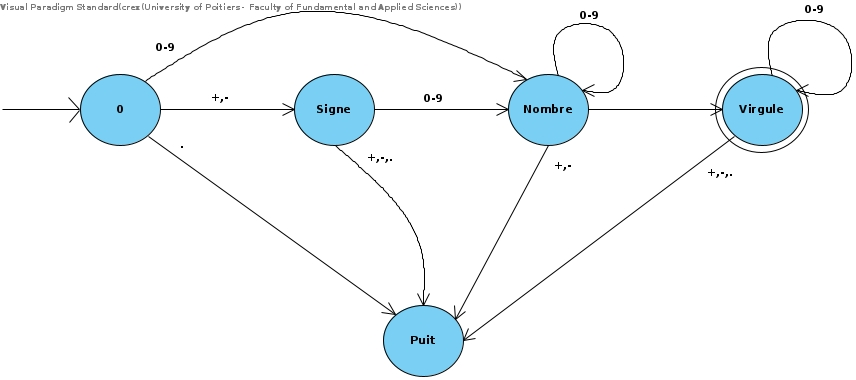
\includegraphics[scale=0.5]{../VP/ex2_2.jpg}
\end{center}
\newpage

%% ---- 3)
\subsubsection{Implantation des reconnaitRec}


%% ---- 4)
\subsubsection{Implantation de l'automate complet}


%% ---- 5)
\subsubsection{Programme complet}



%%%% ======================================= %%%
%%%%                EXERCICE 3               %%%
%%%% ======================================= %%%
%\section{Exercice 3: Des automates non déterministes représentés dans le code de manière récursive}
%
%%% ---- 1)
%\subsubsection{}
%
%
%%% ---- 2)
%\subsubsection{}
%
%
%
%%%% ======================================= %%%
%%%%                EXERCICE 4               %%%
%%%% ======================================= %%%
%\section{Exercice 4: Évaluation du réel correspondant à la chaîne de caractères}
%
%
%%% ---- 1)
%\subsubsection{}
%
%
%%% ---- 2)
%\subsubsection{}
%
%
%%% ---- 3)
%\subsubsection{}
%
%
%%% ---- 4)
%\subsubsection{}

\end{document}